% Set up the document
\documentclass{article}

% Page size
\usepackage[
    letterpaper,]{geometry}

% Lines between paragraphs
\setlength{\parskip}{\baselineskip}
\setlength{\parindent}{0pt}

% Math
\usepackage{mathtools}
\usepackage{amssymb}
\usepackage{commath}

% Math notation macros
\def\*#1{\mathbf{#1}}
\newcommand{\dadvd}[2]{\dfrac{\text{D} #1}{\text{D} #2}} % advective derivative

\newcommand{\fS}{\mathcal{S}} % fancy S
\newcommand{\tphi}{\tilde{\phi}}
\newcommand{\nhat}{\mathbf{\hat{n}}}
\newcommand{\rhat}{\mathbf{\hat{r}}}
\newcommand{\thetahat}{\boldsymbol{\hat{\theta}}}
\newcommand{\xhat}{\mathbf{\hat{x}}}
\newcommand{\yhat}{\mathbf{\hat{y}}}
\newcommand{\zhat}{\mathbf{\hat{z}}}
\newcommand{\omegavec}{\boldsymbol{\omega}}

% Links
\usepackage{hyperref}

% Page numbers at top right
\usepackage{fancyhdr}
\pagestyle{fancy}
\fancyhf{}
\fancyhead[R]{\thepage}
\renewcommand\headrulewidth{0pt}

% Graphics
\usepackage{float}
\usepackage{graphicx}
\graphicspath{ {./img/} }

\begin{document}

\textbf{MATH 462 Assignment 6} \\
\textbf{Matt Wiens \#301294492} \\
\textbf{2020-02-26}

\textbf{A) Flow around an island.} (4 pages + plot) The 2D velocity
potential $\phi(x, y)$ satisfies the Laplace PDE $\nabla^2 \phi = 0$. In
this problem, you will find a harmonic function on an annulus domain $1
\leq r \leq R$ where the BCs are applied as flow velocities normal to
circles at $r = 1$ and $r = R$. For the inner circle, there is no flow:
$\rhat \cdot \*u(1, \theta) = 0$; for the outer circle, the flow is
%
\begin{equation*}
    \rhat \cdot \*u(R, \theta) =
        \begin{cases}
            -1, & 0 < \theta < \pi / 4 \\
            1, & \alpha < \theta < \alpha + \pi / 4 \\
            0, & \text{otherwise}
        \end{cases}
\end{equation*}
%
which specifies inflow ($0 < \theta < \pi / 4$) and outflow ($\alpha <
\theta < \alpha + \pi / 4$) velocity sectors. On the assignment page
there is a sample plot of the streamlines and contours of velocity
potential, along with code for generating it..

\textbf{i)} Using either the method of separation of variables, or a
Fourier construction in $\theta$, present a derivation for the general
solution $\phi(r, \theta)$ for this polar geometry. The two parts to
emphasize are obtaining ODEs for the radial dependence, and integrations
that determine the series coefficients from the BCs. Not that the flow
velocity \textit{cannot} be uniquely determined.

\textbf{ii)} Find the corresponding streamfunction (the harmonic
conjugate) from C-R considerations.

\textbf{iii)} For your own choice of $\alpha$, make a plot of the
streamlines and contours of velocity potential ($R = 2$ makes a nice
plot, but seems not to matter) for the unique solution with zero
circulation. On your plot, indicate regions of fast/slow flow (include
explanations). Also indicate regions of high/low pressure as deduced by
flow curvature (again, include logic).

\textbf{iv)} For your specific choice of $\alpha$, what fraction of the
flow is diverted above, versus below, the island? Explain.

\textbf{Extra plots:} Some intriguing behaviour occurs if enough
circulation is allowed in the solution. Investigate and explain.

\textbf{Bonus:} Your solution method is doomed if the angle of the
outlet sector doesn't match that of the inlet. Explain in terms of the
fluid physics and the mathematics.

\newpage

\textbf{Solution} (Note that I worked with Paul Bologea on this.)

\textbf{i)} The Laplace PDE for $\phi$ in polar coordinates gives us
%
\begin{equation}
    \phi_{\theta \theta} + r \phi_r +  r^2 \phi_{r r} = 0
    \label{eq:A-lap}
\end{equation}
%
Since we are given Neumann boundary conditions, we can solve for $\phi$
using a sine series:
%
\begin{equation}
    \phi(r, \theta) = \sum_{n = 1}^\infty a_n(r) \sin \del{\frac{n \theta}{2}}
    \label{eq:A-setup}
    .
\end{equation}
%
Substituting \eqref{eq:A-setup} into~\eqref{eq:A-lap} we have
%
\begin{equation*}
    \sum_{n = 1}^\infty \del{
        r^2 a_n^{\prime \prime}(r) + r a_n^\prime(r) - \frac{n^2}{4} a_n(r)
    } \sin \del{\frac{n \theta}{2}}
    = 0
    .
\end{equation*}
%
This tells us that for all $n$,
%
\begin{equation}
    r^2 a_n^{\prime \prime}(r) + r a_n^\prime(r) - \frac{n^2}{4} a_n(r) = 0
    \label{eq:A-an}
    .
\end{equation}
%
Now we need to deal with the boundary conditions. Note that $\rhat \cdot
\*u(r, \theta) = \phi_r(r, \theta)$. For the boundary condition at $r =
1$, we clearly get, using~\eqref{eq:A-setup}, that
%
\begin{equation}
    a_n^\prime(1) = 0
    \label{eq:A-bc1}
\end{equation}
%
for all $n$. For the second boundary condition, we need to ``match''
Fourier coefficients with~\eqref{eq:A-setup}. The Fourier coefficients
of the other boundary $b_n$ can be calculated as follows:
%
\begin{align*}
    b_n
        &= \int_0^{2 \pi} \del{\rhat \cdot \*u(R, \theta)} \sin \del{\frac{n \theta}{2}} \dif \theta \\
        &=
            \int_0^{\frac{1}{4}} \sin \del{\frac{n \theta}{2}} \dif \theta
            -
            \int_\alpha^{\frac{\alpha}{4}} \sin \del{\frac{n \theta}{2}} \dif \theta \\
        &=
            \frac{2}{n} \del{1 - \cos \del{\frac{\pi n}{8}}}
            -
            \frac{2}{n} \del{\cos \del{\frac{\alpha n}{2}} - \cos \del{\frac{a n}{2} + \frac{\pi n}{8}}} \\
        &=
            \frac{2}{n} \del{
                1
                - \cos \del{\frac{\pi n}{8}}
                -
                \cos \del{\frac{\alpha n}{2}}
                + \cos \del{\frac{a n}{2} + \frac{\pi n}{8}}
            }
            .
\end{align*}
%
and then we set
%
\begin{equation}
    a_n^\prime(R) = b_n
    \label{eq:A-bc2}
    .
\end{equation}
%
Using Wolfram Alpha, the solution to~\eqref{eq:A-an} together
with~\eqref{eq:A-bc1}~and~\eqref{eq:A-bc2} is
%
\begin{equation}
    a_n(r) = \frac{2 b_n R}{n \del{R^{\frac{n}{2}} - R^{- \frac{n}{2}}}} \del{r^{\frac{n}{2}} + r^{- \frac{n}{2}}}
    \label{eq:A-coeff}
    .
\end{equation}
%
Therefore the solution we obtain using this method is given
by~\eqref{eq:A-setup} together with~\eqref{eq:A-coeff}. Note that this
is not a unique solution to the velocity potential $\phi$, since adding
any linear term in $\theta$ to $\phi$ is valid since it has no bearing
on either the Laplace PDE or the corresponding boundary conditions.

As suggested Dr. Muraki, we will add an additional term $C \theta$ to
the $\phi$ we determined above (where $C \in \mathbb{R}$). Thus the
$\phi$ we use going forward will be
%
\begin{equation}
    \phi(r, \theta) = C \theta
        + \sum_{n = 1}^\infty
            \frac{2 b_n R}{n \del{R^{\frac{n}{2}} - R^{- \frac{n}{2}}}} \del{r^{\frac{n}{2}} + r^{- \frac{n}{2}}}
        \sin \del{\frac{n \theta}{2}}
    .
\end{equation}

\textbf{ii)} Now we need to find the streamfunction $\psi$, the harmonic
conjugate of $\phi$. From the Cauchy-Riemann equations we have
%
\begin{align*}
    \phi_r &= \frac{1}{r} \psi_\theta, \\
    \phi_\theta &= - r \psi_r
    .
\end{align*}
%
Using these equations we can solve for $\psi$. First we have that
%
\begin{align*}
    r \phi_r &=
        r \sum_{n = 1}^\infty
            \frac{b_n R}{\del{R^{\frac{n}{2}} - R^{- \frac{n}{2}}}} \del{r^{\frac{n}{2} - 1} - r^{- \frac{n}{2} - 1}}
        \sin \del{\frac{n \theta}{2}}
        \\
         &= \sum_{n = 1}^\infty
            \frac{b_n R}{\del{R^{\frac{n}{2}} - R^{- \frac{n}{2}}}} \del{r^{\frac{n}{2}} - r^{- \frac{n}{2}}}
        \sin \del{\frac{n \theta}{2}}
        \\
         &= \psi_\theta
         ,
\end{align*}
%
and hence, by integrating with respect to $\theta$, we have
%
\begin{equation}
    \psi(r, \theta)
        = - \sum_{n = 1}^\infty
            \frac{2 b_n R}{n \del{R^{\frac{n}{2}} - R^{- \frac{n}{2}}}} \del{r^{\frac{n}{2}} - r^{- \frac{n}{2}}}
        \cos \del{\frac{n \theta}{2}}
        + c_1(r)
        \label{eq:A-bi}
        ,
\end{equation}
%
where $c_1$ is a constant, possibly depending on $r$. Secondly, we have
%
\begin{align*}
    - \frac{1}{r} \phi_\theta
        &=
            - \frac{1}{r}
            \del{
                C
                + \sum_{n = 1}^\infty
                    \frac{b_n R}{\del{R^{\frac{n}{2}} - R^{- \frac{n}{2}}}} \del{r^{\frac{n}{2}} + r^{- \frac{n}{2}}}
                \cos \del{\frac{n \theta}{2}}
            }
            \\
        &=
            - \del{
                \frac{C}{r}
                + \sum_{n = 1}^\infty
                    \frac{b_n R}{\del{R^{\frac{n}{2}} - R^{- \frac{n}{2}}}} \del{r^{\frac{n}{2} - 1} + r^{- \frac{n}{2} - 1}}
                \cos \del{\frac{n \theta}{2}}
            }
            \\
        &= \psi_r
        .
\end{align*}
%
Integrating with respect to $r$, we have
%
\begin{equation}
    \psi(r, \theta)
        = - C \log r - \sum_{n = 1}^\infty
            \frac{2 b_n R}{n \del{R^{\frac{n}{2}} - R^{- \frac{n}{2}}}} \del{r^{\frac{n}{2}} - r^{- \frac{n}{2}}}
        \cos \del{\frac{n \theta}{2}}
        + c_2(\theta)
        \label{eq:A-bii}
        ,
\end{equation}
%
where $c_2$ is a constant which possibly depends on $\theta$. Taking
together both~\eqref{eq:A-bi} and~\eqref{eq:A-bii}, we have
%
\begin{equation*}
    \psi(r, \theta)
        = - C \log r - \sum_{n = 1}^\infty
            \frac{2 b_n R}{n \del{R^{\frac{n}{2}} - R^{- \frac{n}{2}}}} \del{r^{\frac{n}{2}} - r^{- \frac{n}{2}}}
        \cos \del{\frac{n \theta}{2}}
        .
\end{equation*}
%
\textbf{iii)} First, before discussing anything related to plotting,
let's investigate the circulation for any closed loop in our domain.
Note that in the function $\Phi = \phi + i \psi$ we have the term
%
\begin{equation*}
    C \theta - i C \log r = - i C \log \del{r e^{i \theta}} = - i C \log z
\end{equation*}
%
and hence in the Laurent series for $\dod{\Phi^*}{z}$ in our domain, the $c_{-1}$ term
is $i C$. Thus the circulation along any path $C$ within our domain given by
%
\begin{equation*}
    \Gamma = \Re \cbr{ \oint_C \dod{\Phi^*}{z} \dif z } = 2 \pi i (i C) = - 2 \pi C
    .
\end{equation*}
%
So to produce a plot with no circulation we only need to set $C = 0$.
For the sake of completeness, a plot is included on a following page;
however, the solution is obviously wrong since it is discontinuous at
$\theta = 0$.

However, with that said, if we did have a proper solution, we could
determine regions with fast and slow flow, by the density of
streamlines. For example, in the plot of the doomed solution the flow
speed is highest closest to the center and slower closer to the boundary
at $r = R$. Additionally it appears that the flow speeds are in general
higher on the upper half plane than their corresponding points on the
lower half plane.

Additionally, we can determine regions of higher or lower pressure by
nothing that fluid tends to curve towards regions of lower pressure.
Thus in the doomed solution, we would expect lower pressure in the
centre, and higher pressure away from it.

\textbf{iv)} I'm not 100\% sure what this part is asking for. It appears
that most of the flow is diverted above the island, however.

\newpage

\begin{figure}
    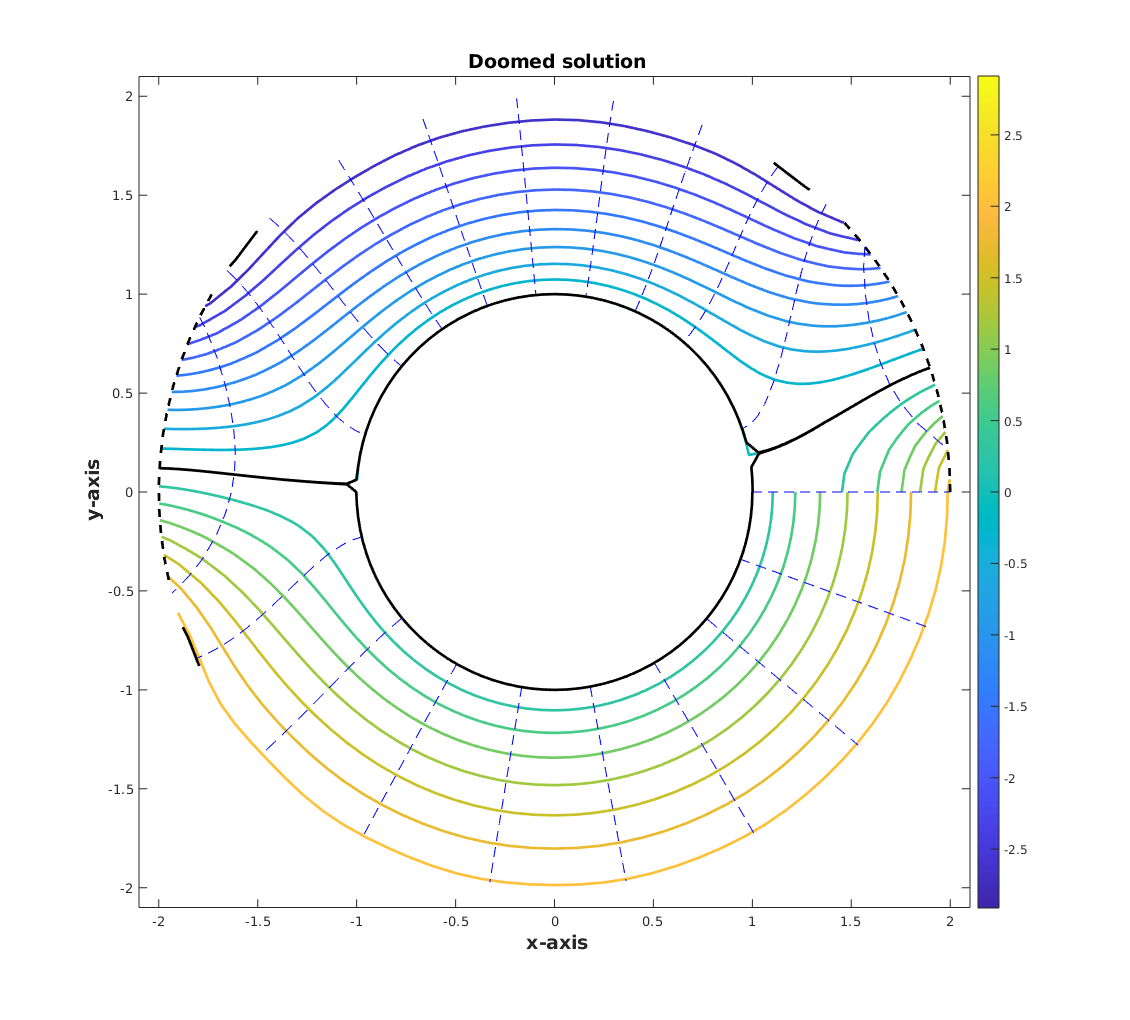
\includegraphics[width=\textwidth]{doomed}
    \centering
\end{figure}

\

\newpage

\textbf{B) Potential flow and branch cuts.} (2 pages + annotated plots)
The included MATLAB script makes contour plots for a complex potential
$\Phi(z)$ that corresponds to flow past a flat plate,
%
\begin{equation*}
    \Phi(z) = (z^2 + 1)^{1/2}
    .
\end{equation*}
%
\textbf{i)} Explain why it is clear that the far-field flow is
uniform (Acheson, p. 135).

\textbf{ii)} Note that the script draws a thick black line representing
the flat plate. But, there is evidence in MATLAB's branch cut in the
``bunched'' dotted contours. To understand MATLAB's branch cut choice for
the square root better, change the script to evaluate $\Phi$ using
%
\begin{equation*}
    \Phi(z) = (z + i)^{1/2} (z - i)^{1/2}
    .
\end{equation*}
%
Now use polar coordinates, as in lecture, to explain how MATLAB chooses
its square root branch cut.

\textbf{iii)} An additional caution arises when you are asked to take
the derivative of $\Phi$ to evaluate the velocities
%
\begin{equation*}
    \dod{\Phi}{z} = u(x, y) - i v(x, y)
    .
\end{equation*}
%
It is almost never taught how to think about differentiation in the
presence of a branch choice. The proper power rule for $z^n$ is
%
\begin{equation*}
    \dod{}{z} z^n = n \frac{z^n}{z}
    ,
\end{equation*}
%
where the branch choice is the same as for the function evaluation of
$z^n$. Derive the velocity formulas and modify a previous (quiver)
script to show that the branch cut discontinuity of $\Phi$ does not
affect the continuity of the flow arrows (property 4b-iii from lecture).

\textbf{iv)} Finally, the MATLAB finesse for this flow problem is to
define instead
%
\begin{equation*}
    \Phi(z) = -i (i z + 1)^{1/2} (i z - i)^{1/2}
    .
\end{equation*}
%
Change the script to show that now the branch cut is exactly along the
flat plate (property 4b-i from lecture).

\textbf{v)} Note that this type of flow makes an appearance in
Sebastian's parking lot video that is posted on the lecture notes page
(week 3). Include a zoomed-in snapshot of this feature in your
submission.

\textbf{Extra:} Explain why the branch cut appears where it does for the
original expression for $\Phi(z)$. This might be difficult.

\newpage

\textbf{Solution.}

Note to self: don't leave homework for the day it's due.

\end{document}
